\documentclass[final]{article}
\usepackage[paperwidth=48in,paperheight=36in,margin=0.45in]{geometry}
\usepackage[utf8]{inputenc}
\usepackage[T1]{fontenc}
\usepackage{lmodern}
\usepackage{xcolor}
\usepackage{graphicx}
\usepackage{array}
\usepackage{tabularx}
\usepackage{hyperref}
\pagestyle{empty}

\definecolor{Ink}{HTML}{18202A}
\definecolor{Muted}{HTML}{516071}
\definecolor{Paper}{HTML}{F7F5EF}
\definecolor{Panel}{HTML}{FFFFFF}
\definecolor{Line}{HTML}{D7D0C2}
\definecolor{Blue}{HTML}{315F85}
\definecolor{Green}{HTML}{37715F}
\definecolor{Red}{HTML}{9A4C4C}
\definecolor{Gold}{HTML}{BD8A33}
\definecolor{SoftBlue}{HTML}{E8F0F5}
\definecolor{SoftGreen}{HTML}{F0F8F4}
\definecolor{SoftGold}{HTML}{FFF7DF}
\definecolor{SoftRed}{HTML}{F9ECE8}

\hypersetup{colorlinks=true,urlcolor=Blue}
\renewcommand{\familydefault}{\sfdefault}
\setlength{\parindent}{0pt}
\setlength{\parskip}{0.15in}
\setlength{\fboxsep}{0.16in}
\setlength{\fboxrule}{1.1pt}

\newcommand{\TitleText}[1]{{\fontsize{86}{88}\selectfont\bfseries #1}}
\newcommand{\SubTitle}[1]{{\fontsize{25}{31}\selectfont #1}}
\newcommand{\Section}[1]{{\color{Gold}\rule{0.18in}{0.48in}}\hspace{0.12in}{\fontsize{25}{28}\selectfont\bfseries\color{Blue} #1}\par\vspace{0.05in}}
\newcommand{\SmallSection}[1]{{\fontsize{19}{22}\selectfont\bfseries\color{Blue} #1}\par\vspace{0.04in}}
\newcommand{\Body}[1]{{\fontsize{15.5}{20}\selectfont\color{Muted} #1\par}}
\newcommand{\BodyTight}[1]{{\fontsize{14.5}{18}\selectfont\color{Muted} #1\par}}
\newcommand{\Key}[1]{{\fontsize{18}{23}\selectfont\bfseries\color{Ink} #1\par}}
\newcommand{\Panel}[1]{\fcolorbox{Line}{Panel}{\begin{minipage}[t]{0.955\linewidth}#1\end{minipage}}}
\newcommand{\MiniPanel}[2]{%
  \fcolorbox{#1}{#2}{\begin{minipage}[t]{0.92\linewidth}#2\end{minipage}}%
}
\newcommand{\Metric}[3]{%
  \fcolorbox{Line}{SoftGold}{%
    \begin{minipage}[c][1.05in][c]{#1}
      \centering
      {\fontsize{34}{35}\selectfont\bfseries\color{Green} #2}\par
      {\fontsize{12}{14}\selectfont\bfseries\color{Muted} #3}
    \end{minipage}
  }
}
\newcommand{\Tag}[2]{%
  \fcolorbox{#1}{#2}{\begin{minipage}[c][0.55in][c]{0.92\linewidth}{\fontsize{14}{17}\selectfont\bfseries\color{Ink} #2}\end{minipage}}%
}
\newcommand{\Finding}[1]{%
  \fcolorbox{Green}{SoftGreen}{\begin{minipage}[t]{0.91\linewidth}{\fontsize{14.5}{18}\selectfont\bfseries\color{Green} #1}\end{minipage}}\par\vspace{0.1in}
}

\begin{document}
\pagecolor{Paper}
\color{Ink}

\colorbox{Blue}{%
  \begin{minipage}[c][3.15in][c]{0.985\linewidth}
    \hspace{0.18in}
    \begin{minipage}[c]{0.66\linewidth}
      {\color{white}\TitleText{Writing Helper}}\par
      \vspace{0.12in}
      {\color{white}\SubTitle{Interruption-aware AI writing that learns a transparent style profile from stop points, repairs, and repeated revision choices.}}
    \end{minipage}
    \hfill
    \begin{minipage}[c]{0.285\linewidth}
      \fcolorbox{white}{SoftGold}{%
        \begin{minipage}[c][2.28in][c]{0.92\linewidth}
          {\fontsize{13}{15}\selectfont\bfseries\color{Muted} CENTRAL CLAIM}\par
          {\fontsize{42}{44}\selectfont\bfseries\color{Red} Stop = Signal}\par
          {\fontsize{17}{21}\selectfont\color{Ink} A writer's interruption is not just a cancellation; it is evidence about voice, specificity, structure, and argument.}
        \end{minipage}
      }
    \end{minipage}
    \hspace{0.18in}
  \end{minipage}
}

\vspace{0.28in}

\begin{minipage}[t]{0.24\linewidth}
\Panel{
  \Section{Introduction}
  \Key{Fluent AI prose can still feel wrong.}
  \Body{Writing Helper is a local browser prototype for interruption-aware multi-agent writing. When the user stops a generated sentence and chooses a better repair, the system treats that behavior as preference evidence.}
  \fcolorbox{Blue}{SoftBlue}{\begin{minipage}{0.91\linewidth}{\fontsize{17}{22}\selectfont\bfseries\color{Blue} Research question: Can interruption behavior recover latent preferences about wording, tone, structure, specificity, and argumentative style?}\end{minipage}}
}

\vspace{0.18in}
\Panel{
  \Section{Motivation}
  \Body{Prompt-based personalization asks users to articulate their style in advance. This creates extra labor and favors strong prompt engineers.}
  \Body{This prototype learns from ordinary revision behavior: stop when a sentence feels wrong, choose or write a better option, and let repeated choices become inspectable memory.}
  \fcolorbox{Red}{SoftRed}{\begin{minipage}{0.91\linewidth}{\fontsize{16}{20}\selectfont\bfseries\color{Red} Design goal: turn dissatisfaction into a durable, editable writing profile.}\end{minipage}}
}

\vspace{0.18in}
\Panel{
  \Section{What It Contributes}
  {\fontsize{14.4}{18}\selectfont\color{Muted}
  \begin{itemize}
    \setlength\itemsep{0.04in}
    \item Behavior-first personalization from interruption and repair.
    \item Inspectable profile memory rather than hidden adaptation.
    \item Local profile storage, revision log, and audit export.
    \item Promotion rule: repeated evidence before durable memory.
  \end{itemize}}
}

\vspace{0.18in}
\Panel{
  \Section{Simulation Design}
  \BodyTight{Each fake user receives a hidden profile drawn from wording, voice, style, and structure preferences. The assistant only observes interruptions and repairs, not the hidden profile itself.}
  \BodyTight{A profile item is promoted only after three similar observations, which intentionally delays recall but reduces one-click overfitting.}
}
\end{minipage}
\hfill
\begin{minipage}[t]{0.24\linewidth}
\Panel{
  \Section{Process Pipeline}
  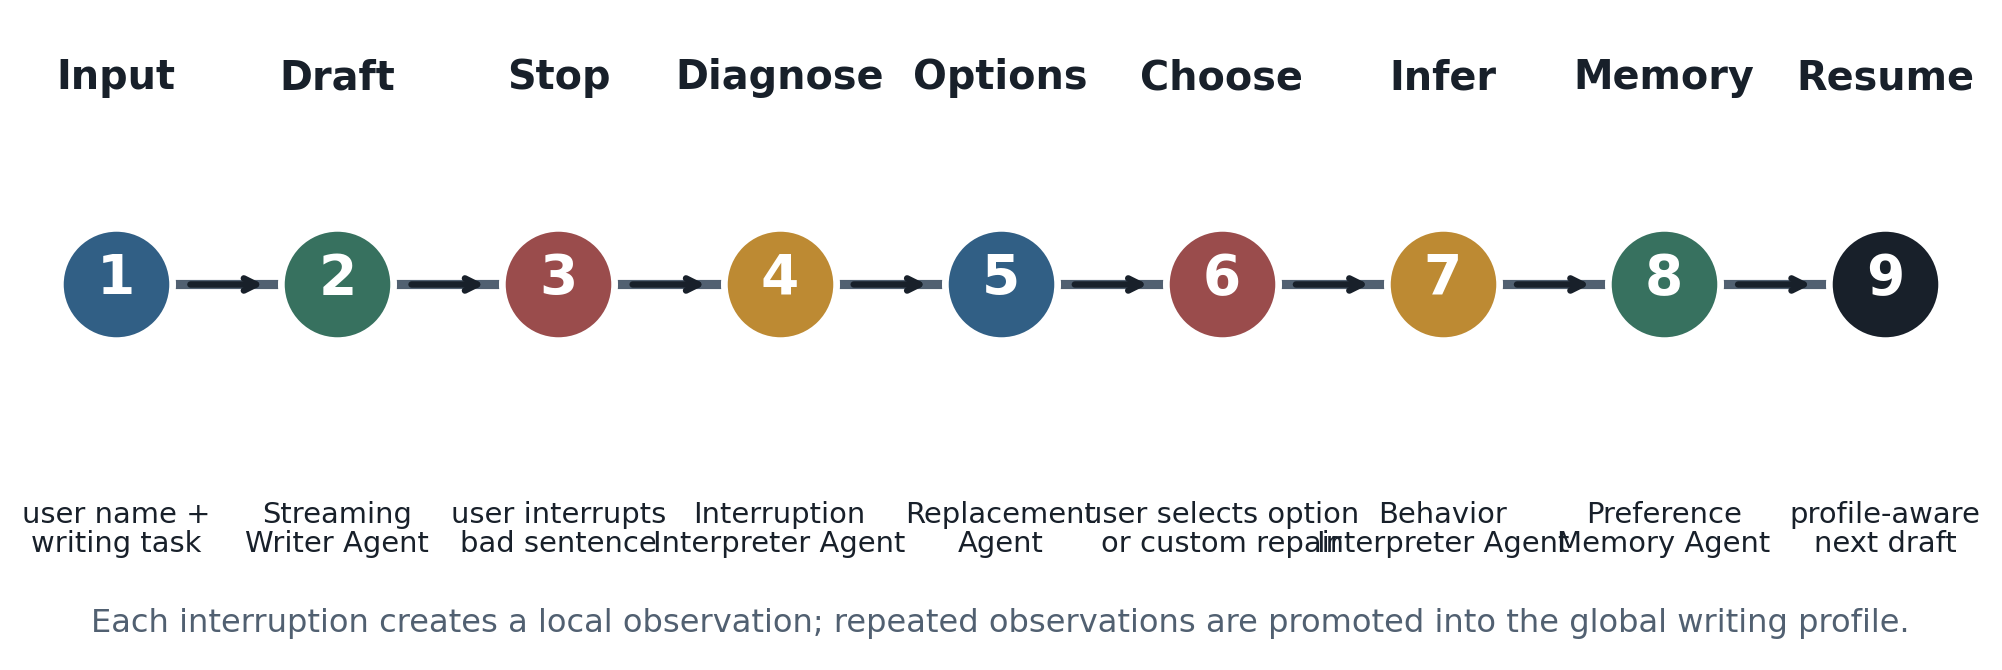
\includegraphics[width=\linewidth]{poster_pipeline.png}
  \vspace{0.05in}
  \BodyTight{The pipeline begins with explicit user input, then alternates between agent work and user feedback. Each repair produces an observation that can later become profile memory.}
}

\vspace{0.18in}
\Panel{
  \Section{Agents Involved}
  {\fontsize{14.2}{17.5}\selectfont\color{Muted}
  \begin{tabularx}{\linewidth}{>{\bfseries\color{Ink}}p{1.55in} X}
    Streaming Writer & drafts and resumes generation.\\
    Interruption Interpreter & explains why the stopped sentence may feel wrong.\\
    Replacement Agent & proposes candidate rewrites.\\
    Behavior Interpreter & interprets custom user feedback.\\
    Preference Memory & records local hints and promotes repeated preferences.
  \end{tabularx}}
}

\vspace{0.18in}
\Panel{
  \Section{Example Trace}
  \BodyTight{\textbf{\color{Red} Interrupted draft:} ``Bioethics is a broad field that deals with medicine, technology, public health, and social values.''}
  \BodyTight{\textbf{\color{Blue} Chosen repair reason:} Match latent style: avoid generic academic filler.}
  \BodyTight{\textbf{\color{Green} Memory update:} observation 1/3; kept local until the same preference appears repeatedly.}
  \BodyTight{\textbf{\color{Gold} Later promotion:} after a third similar choice, ``avoid generic academic filler'' enters the global profile.}
}

\vspace{0.18in}
\Panel{
  \Section{Data}
  \Metric{0.29\linewidth}{100}{simulated writers}\hfill
  \Metric{0.29\linewidth}{30}{steps each}\hfill
  \Metric{0.29\linewidth}{2486}{interruptions}
  \vspace{0.12in}
  \Metric{0.29\linewidth}{512}{manual actions}\hfill
  \Metric{0.29\linewidth}{10.47}{target items}\hfill
  \Metric{0.29\linewidth}{5.00}{recovered items}
}
\end{minipage}
\hfill
\begin{minipage}[t]{0.24\linewidth}
\Panel{
  \Section{Results}
  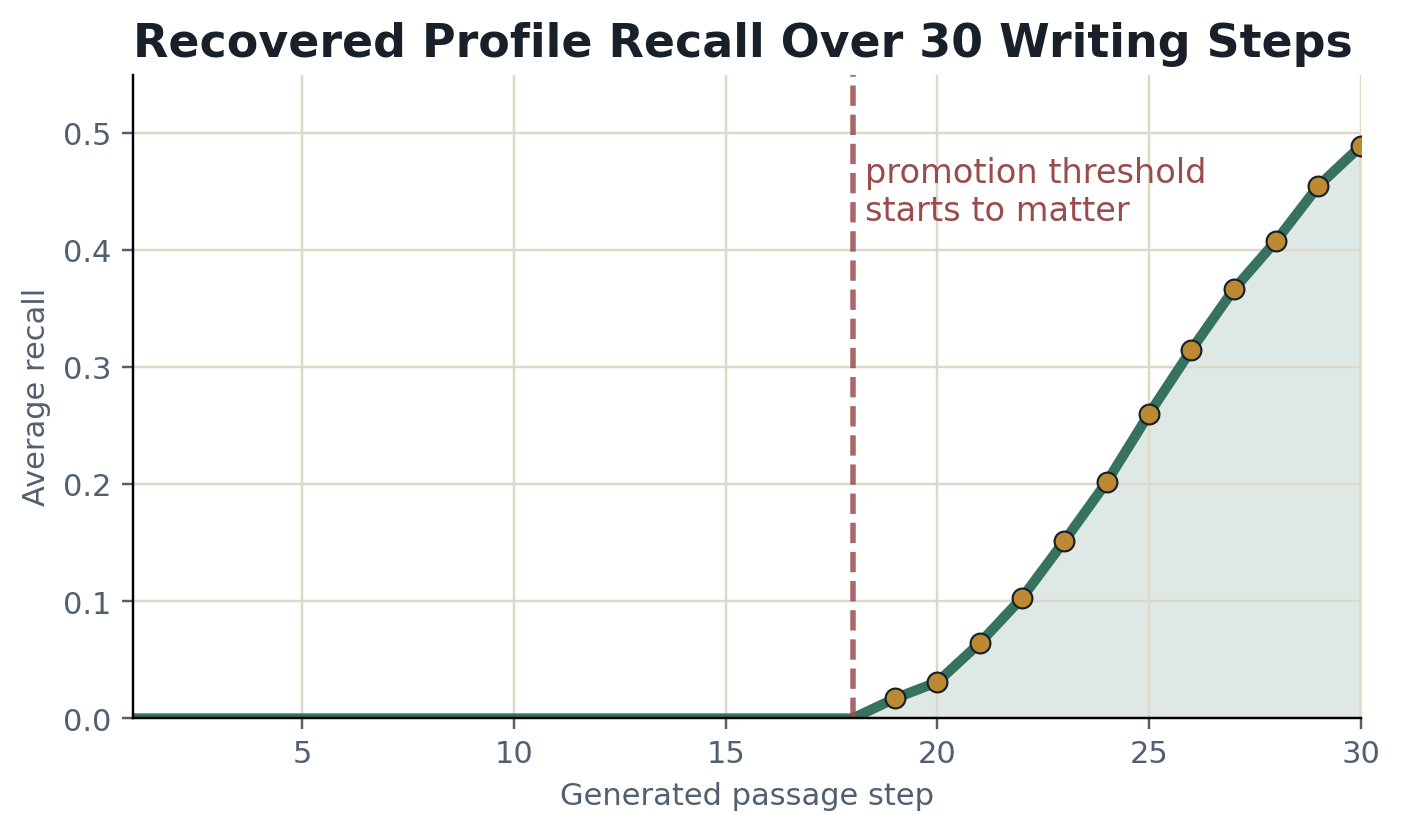
\includegraphics[width=\linewidth]{poster_recovery_curve.png}
  \vspace{0.05in}
  \Metric{0.30\linewidth}{0.489}{mean final recall}\hfill
  \Metric{0.30\linewidth}{0.495}{median final recall}\hfill
  \Metric{0.30\linewidth}{0.923}{max recall}
}

\vspace{0.18in}
\Panel{
  \Section{Promotions}
  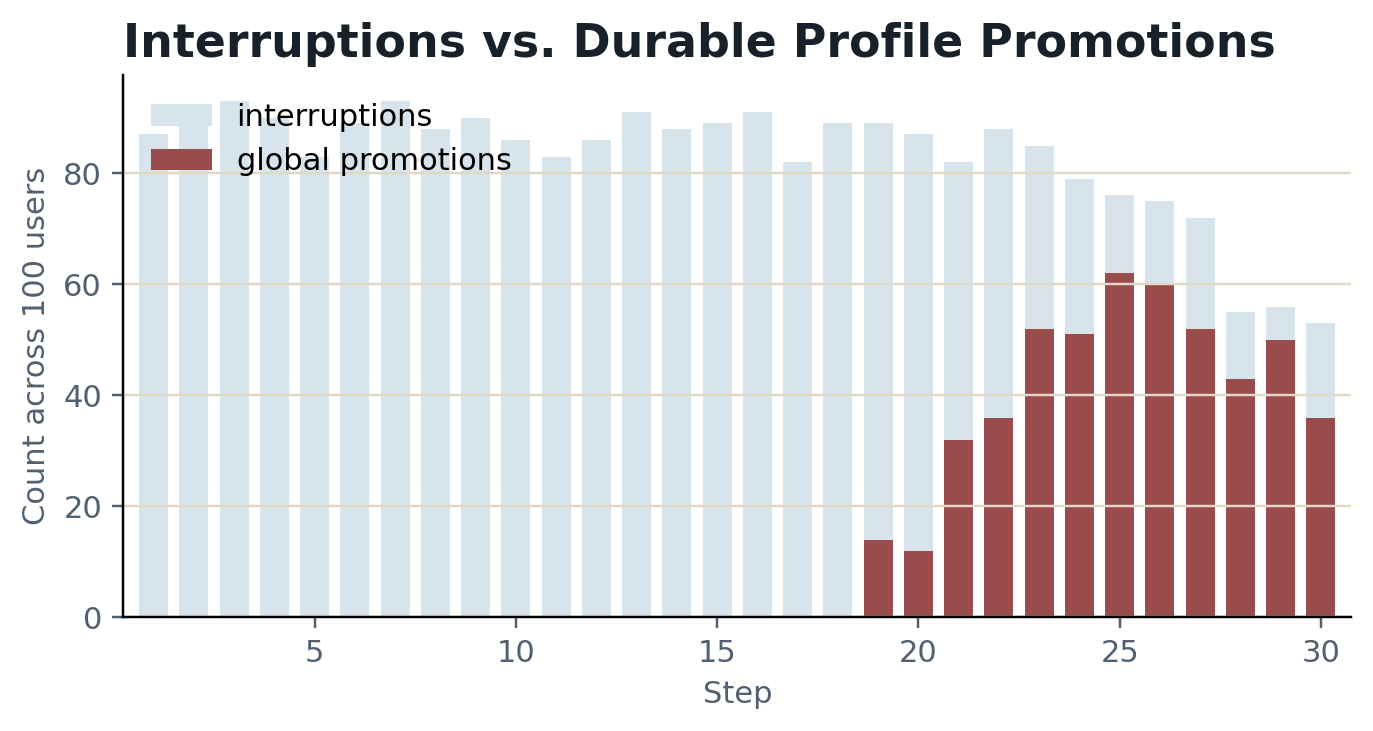
\includegraphics[width=\linewidth]{poster_promotion_bars.png}
  \BodyTight{The system interrupts often, but durable profile updates appear later because a preference must recur before promotion.}
}

\vspace{0.18in}
\Panel{
  \Section{Action Mix}
  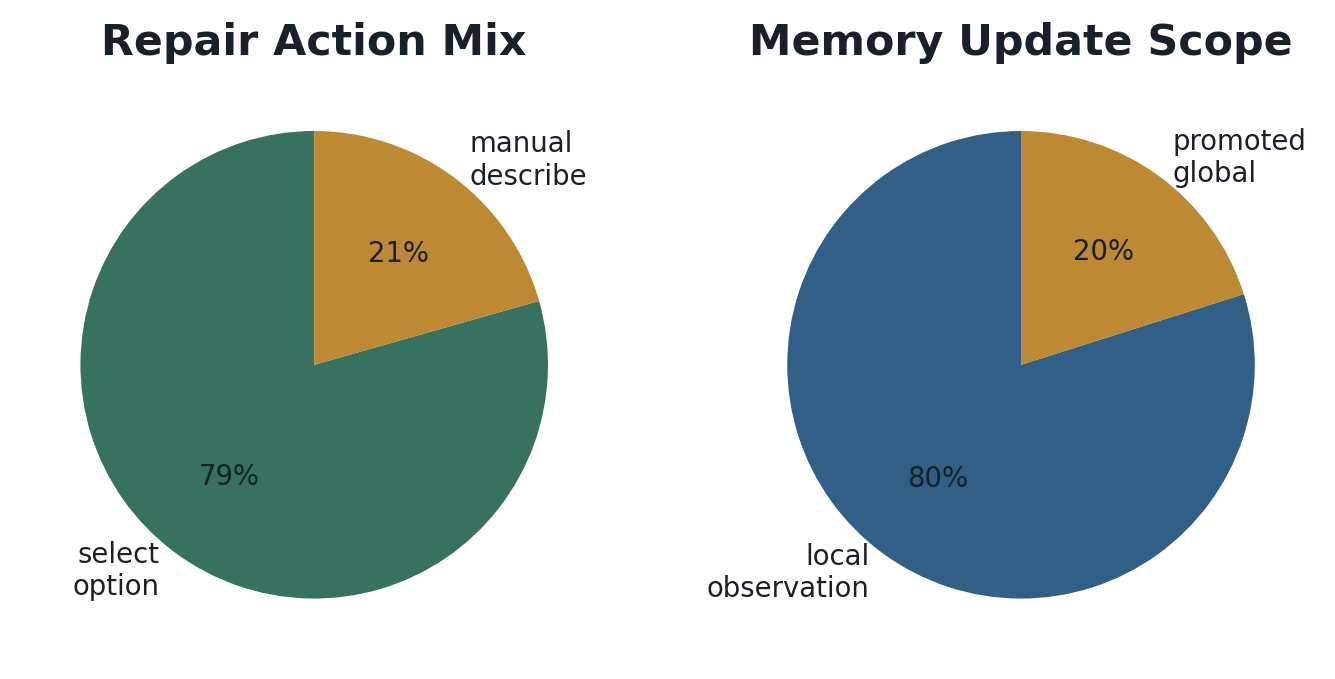
\includegraphics[width=\linewidth]{poster_action_mix.png}
}

\vspace{0.18in}
\Panel{
  \Section{Result Reading}
  \BodyTight{The curve is intentionally flat at first because the memory module requires repeated evidence. After step 18, repeated repairs begin converting local observations into global style memory.}
}
\end{minipage}
\hfill
\begin{minipage}[t]{0.24\linewidth}
\Panel{
  \Section{Hidden Preferences}
  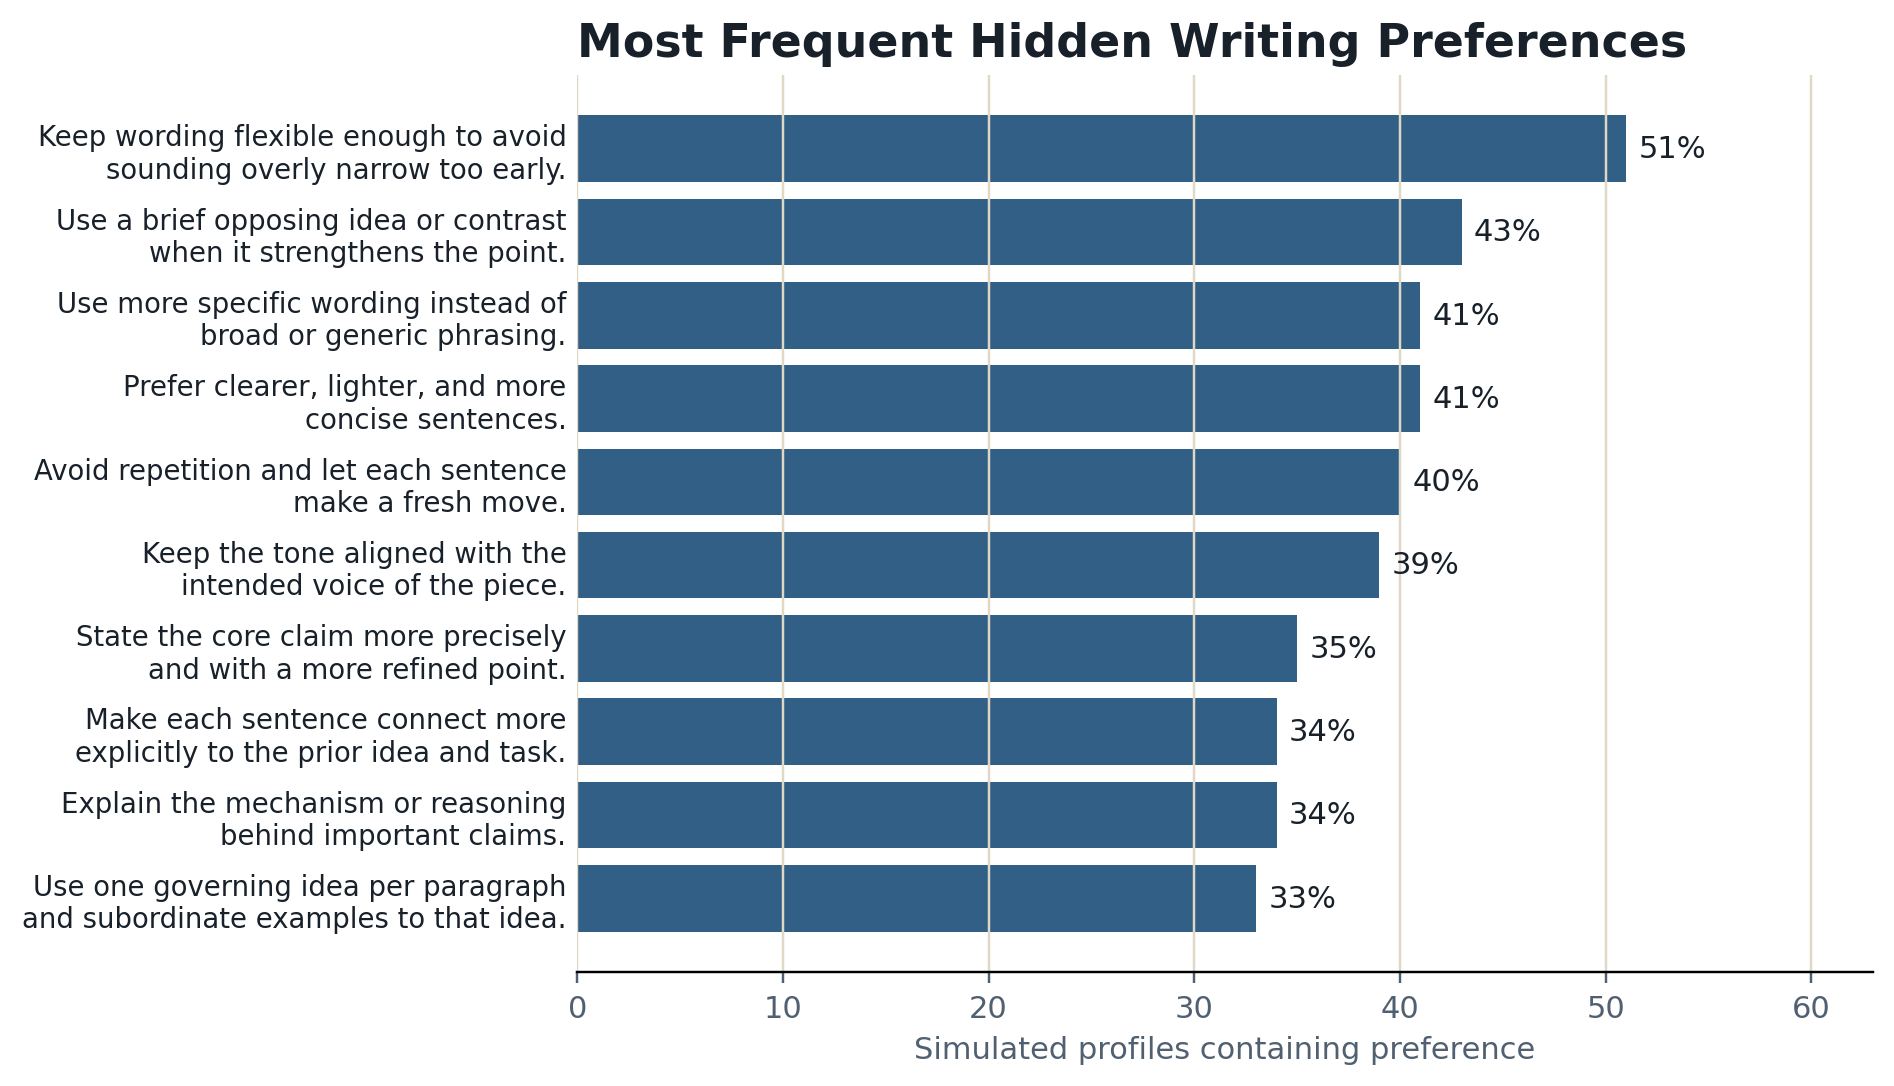
\includegraphics[width=\linewidth]{poster_profile_frequency.png}
}

\vspace{0.18in}
\Panel{
  \Section{Interpretation}
  \Finding{Low early recall is expected: one click is treated as weak local evidence.}
  \Finding{The late rise shows that repeated stop-and-repair behavior can recover stable style preferences.}
  \Finding{The run validates the logging and recovery pipeline, but it is still an offline simulation rather than a human study.}
  \Finding{The next evaluation should compare recovered profiles against real writers' self-reported style preferences.}
}
\end{minipage}

\vspace{0.22in}

\fcolorbox{Line}{Panel}{%
  \begin{minipage}[t]{0.975\linewidth}
    \Section{References Leading To This Work}
    \begin{minipage}[t]{0.49\linewidth}
      {\fontsize{14.5}{18}\selectfont\color{Muted}
      \textbf{\color{Ink}CoAuthor.} Lee, M., Liang, P., and Yang, Q. (2022). \textit{CoAuthor: Designing a Human-AI Collaborative Writing Dataset for Exploring Language Model Capabilities.} The present work follows CoAuthor's insight that interaction traces, not only final text, reveal how people collaborate with language models. \url{https://arxiv.org/abs/2201.06796}}
    \end{minipage}
    \hfill
    \begin{minipage}[t]{0.49\linewidth}
      {\fontsize{14.5}{18}\selectfont\color{Muted}
      \textbf{\color{Ink}GhostWriter.} Yeh, C., Ramos, G., Ng, R., Huntington, K., and Banks, R. (2024). \textit{GhostWriter: Augmenting Collaborative Human-AI Writing Experiences Through Personalization and Agency.} Writing Helper narrows the personalization question to interruption points and selected repairs as style-learning evidence. \url{https://arxiv.org/abs/2402.08855}}
    \end{minipage}
  \end{minipage}
}

\vspace{0.1in}
\begin{center}
{\fontsize{13}{16}\selectfont\color{Muted} Local prototype: streaming writer agent + interruption interpreter + replacement agent + transparent preference memory. Data source: deterministic offline recovery run in \texttt{docs/poster\_simulation.json}.}
\end{center}

\end{document}
